\chapter*{Segmentace obrazu} \label{sec:segmentace_obrazu}

Předpokládejme, že máme obraz, který je popsán obrazovou funkcí, a že máme rozpoznat objekty v tomto obraze. Prvním krokem k tomuto cíli je extrakce objektů, které se v obraze nacházejí. Proces extrakce, v němž jsou objekty separovány od nezajímavého pozadí, nazýváme segmentací obrazu. Segmentace je nejčastěji založena na detekci kontur (hran) ohraničujících jednotlivé objekty nebo na detekci celých oblastí, kterými jsou jednotlivé objekty v obraze reprezentovány. Oba uvedené postupy jsou v praxi široce používány, a proto jsou jejich popisu věnovány poměrně rozsáhlé podkapitoly \ref{sec:detekce_hran}, XXX, XXX. V podkapitolách XXX, \ref{sec:zpracovani_binarnich_obrazu} je pak stručně nastíněna problematika detekce rohů objektů a problematika zpracování binárních obrazů.

\section*{Detekce hran} \label{sec:detekce_hran}

Představujeme si, že každý objekt je v obraze reprezentován souvislou oblastí (obr. \ref{img:8_1}a). Každá oblast je obklopena hranicí. Hranice se skládá z hran (případně též z jediné zakřivené hrany). Hrana se skládá z jednotlivých bodů. Významným problémem v analýze obrazů je nalezení hran a celých hranic. Při řešení se často postupuje tak, že se nejprve naleznou jednotlivé body hran. Uvažujme pro jednoduchost obrazy ve stupních šedi. Na existenci bodu hrany můžeme usuzovat z průběhu obrazové funkce. Na obr. \ref{img:8_2} nahoře je znázorněn typický průběh jasu napříč hranou. Za bod hrany se nejčastěji považuje místo, kde průběh jasu vykazuje náhlou změnu, případně inflexní bod. Jednotlivé nalezené body hran jsou pak různými technikami spojovány do hran a celých hranic. Protože každá plocha by měla být obklopena svojí hranicí (obr. \ref{img:8_1}), zdá se, že detekce hran a detekce celých ploch by teoreticky měly vést ke vzájemně ekvivalentním výsledkům. V praxi se však mohou vyskytnout problémy: Jsou-li např. rozpoznávané objekty v obraze špatně zřetelné nebo je-li obraz poškozen šumem, pak nemusí nalezené hrany tvořit kolem objektů uzavřené smyčky, jak si teoreticky představujeme. Vlivem šumu mohou být na druhé straně hrany detekovány i tam, kde ve skutečnosti nejsou.

\begin{figure}[th]
    \begin{center}
        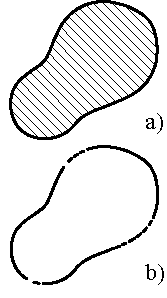
\includegraphics[scale=1.0]{08_segmentace/images/img_8_1.pdf}
    \end{center}
    \caption{Detekce oblastí stanovením hranice.}
    \label{img:8_1}
\end{figure}

\subsection*{Gradientní metody hledání hran}

Obr. \ref{img:8_2} ukazuje typický průběh jasu ve směru napříč hranou a první a druhou derivaci tohoto průběhu. Gradientní metody využívají skutečnosti, že v místě hrany má absolutní hodnota první derivace průběhu jasu vysokou hodnotu. Hodnota derivace popisuje intenzitu kontury v daném bodě - hovoříme o velikosti hrany. Operátory, které velikost hrany stanovují (obvykle se aplikují v každém bodě obrazu), bývají nazývány hranovými operátory. Z uvedeného vyplývá, že nejjednoduššími hranovými operátory jsou zřejmě derivace $\partial$\textit{f}/$\partial$\textit{x} a $\partial$\textit{f}/$\partial$\textit{y}, které popisují změnu úrovně jasu ve směru os \textit{x} a \textit{y}. Těchto operátorů by bylo možné použít k hledání hran rovnoběžných se souřadnými osami. Při hledání hran obecného směru je zapotřebí vyšetřovat průběh jasu ve směru kolmém na směr potenciální hrany. Nechť vektor \textbf{n} = ($\cos \theta$, $\sin \theta$) popisuje směr kolmý ke směru eventuální hrany a $\xi$ nechť je souřadnice měřená v tomto směru. K ověření skutečnosti, zda v daném bodě existuje hrana známého směru, lze použít derivaci ve směru. Pro derivaci ve směru kolmo k hraně máme

\begin{equation} \label{eq:8_1}
    \frac{\partial f}{\partial \xi} = \mathrm{grad} (f) \cdot \mathbf{n} = \frac{\partial f}{\partial x} \cos \theta + \frac{\partial f}{\partial y} \sin \theta .
\end{equation}

\begin{figure}[th]
    \begin{center}
        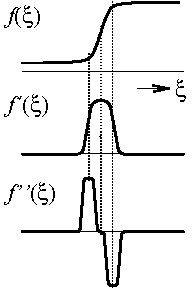
\includegraphics[scale=1.0]{08_segmentace/images/img_8_2.pdf}
    \end{center}
    \caption{Průběh jasu a jeho první a druhé derivace v místě hrany.}
    \label{img:8_2}
\end{figure}

Za velikost hrany v daném bodě můžeme považovat hodnotu \textbar $\partial$\textit{f}/$\partial$$\xi$\textbar . Při hledání hrany její směr předem obvykle neznáme. Rovnice \eqref{eq:8_1} a úvahy, které k ní vedly, však podávají návod, jak situaci řešit. Pro rozhodnutí, zda ve vyšetřovaném bodě je či není hrana, bude rozhodující směr, v němž je změna jasu největší. Tímto směrem je gradient obrazové funkce. Směr hrany je pak kolmý ke směru gradientu. Za velikost hrany lze vzít velikost gradientu. Označme \textit{e}(\textit{x},\textit{y}) velikost hrany, $\varphi$(\textit{x},\textit{y}) směr gradientu a $\psi$(\textit{x},\textit{y}) směr hrany v bodě (\textit{x},\textit{y}). Dále pro stručnost zaveďme značení  \textit{fx}(\textit{x},\textit{y}) = $\partial$\textit{f} (\textit{x},\textit{y})/$\partial$\textit{x},  \textit{fy}(\textit{x},\textit{y}) = $\partial$\textit{f} (\textit{x},\textit{y})/$\partial$\textit{y}. Pak máme:

\begin{equation} \label{eq:8_2}
    e(x, y) = \sqrt{ f_x^2(x, y) + f_y^2(x, y)},
\end{equation}

\begin{equation} \label{eq:8_3}
    \varphi(x, y) = \arctan \left[ \frac{f_x^2(x, y)}{f_y^2(x, y)} \right], \quad \Psi(x, y) = \varphi(x, y) + \frac{\pi}{2} .
\end{equation}

\begin{figure}[th]
    \begin{center}
        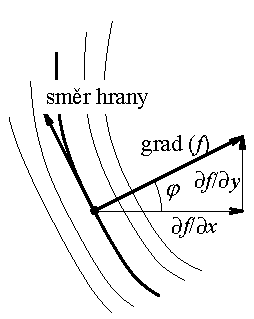
\includegraphics[scale=1.0]{08_segmentace/images/img_8_3.pdf}
    \end{center}
    \caption{Stanovení velikosti a směru hrany na základě gradientu.}
    \label{img:8_3}
\end{figure}

Cílem praktického výpočtu zpravidla bývá rozhodnout, zda vyšetřovaný bod obrazu je či není bodem ležícím na hranici nějakého objektu. V nejjednodušším případě lze za body hranice považovat ta místa, kde hodnota \textit{e}(\textit{x},\textit{y}) je větší než nějaká pevná, předem zvolená prahová hodnota. Tento jednoduchý postup má ovšem své nedostatky: 1) Hranice objektu obvykle vyjde silnější než jeden bod (intuitivně si možná představujeme, že tloušťka hranice je právě jeden bod). 2) Uvedený postup neřeší problém doplnění chybějících a odstranění nadbytečných částí hranice diskutovaný v úvodu podkapitoly \ref{sec:detekce_hran}. Důmyslnější postupy popíšeme postupně později (např. v souvislosti s Cannyho detektorem hran).

Až dosud jsme předpokládali, že obrazová funkce je spojitá. Při praktické implementaci pracujeme ovšem nejčastěji s funkcí diskrétní. Jestliže nahradíme derivace diferencemi, můžeme vztahů \eqref{eq:8_2}, \eqref{eq:8_3} snadno použít i pro diskrétní případ. Pro diference můžeme psát

\begin{equation} \label{eq:8_4}
    f_x(x, y) = f(x + 1, y) - f(x, y),
\end{equation}

\begin{equation} \label{eq:8_5}
    f_y(x, y) = f(x, y + 1) - f(x, y).
\end{equation}

Při praktické realizaci výpočtu je hodnota \textit{e}(\textit{x},\textit{y}) stanovována a porovnávána s hodnotou prahu ve všech bodech (pixelech) obrazu. Poznamenejme, že při stanovení délky gradientu lze použít i jiných metrik, než je metrika uvedená ve vztahu \eqref{eq:8_2} (kořeny těchto snah sahají ovšem poněkud do minulosti, kdy byl výpočet odmocniny časově velmi náročnou, a proto obávanou operací). Můžeme použít např. následujících vztahů:

\begin{equation} \label{eq:8_6}
    e(x, y) = | f_x(x, y) | + | f_y(x, y) |, \quad e(x, y) = \max \left\{ | f_x(x, y) |, | f_y(x, y) | \right\}.
\end{equation}

Skutečnost, že při praktickém výpočtu na použité metrice příliš nezáleží, ukazuje následující příklad, který ponecháváme čtenáři k samostatnému řešení. Příklad: Dokažte, že pro každou dvojici nezáporných čísel \textit{a},\textit{b} platí (\textit{a} + \textit{b})/$\surd$2 $\leq$ $\surd$($a^2$ + $b^2$) $\leq$ $\surd$2 max$\{$\textit{a}, \textit{b}$\}$. 

V minulosti bylo realizováno mnoho praktických metod pro detekci hran, jejichž společným teoretickým základem je výpočet velikosti gradientu. Některé z nich popíšeme dále podrobněji.

\paragraph{Robertsův operátor:} Tento hranový operátor je jedním z nejstarších, ale stále ještě používaným operátorem pro stanovení velikosti hrany. Operátor stanovuje diference ve dvou na sebe kolmých diagonálních směrech. Velikost hrany v bodě (x, y) obrazu se počítá podle předpisu

\begin{equation} \label{eq:8_7} 
    e(x,y)=\sqrt{\left(f(x,y)-f(x+1,y+1)\right)^{2} +\left(f(x+1,y)-f(x,y+1)\right)^{2} } .   
\end{equation}

Někdy také bývá uváděn vztah, v němž jsou místo funkčních hodnot použity jejich odmocniny. Tato varianta údajně více odpovídá vnímání hran lidským zrakem.

\begin{equation} \label{eq:8_8}
    e(x,y)=\sqrt{\left(\sqrt{f(x,y)} -\sqrt{f(x+1,y+1)} \right)^{2} +\left(\sqrt{f(x+1,y)} -\sqrt{f(x,y+1)} \right)^{2} } .   
\end{equation} 

\paragraph{Operátor Prewittové:} Tento operátor využívá k výpočtu velikosti hrany v bodě o souřadnicích $x$, $y$  hodnot obrazové funkce ve všech sousedních pixelech. Tyto hodnoty pro stručnost označíme $A$, $B$, $C$, $D$, $F$, $G$, $H$, $I$ (obr. \ref{img:8_4}). Operátor počítá derivace ve směrech os $x$, $y $průměrem

\begin{equation}
    f_{x} \left(x,y\right)=\frac{1}{3} \left[\left(C-A\right)+\left(F-D\right)+\left(I-G\right)\right], \nonumber
\end{equation} 

\begin{equation} \label{eq:8_9}
f_{y} \left(x,y\right)=\frac{1}{3} \left[\left(A-G\right)+\left(B-H\right)+\left(C-I\right)\right].  
\end{equation}

\begin{figure}[th]
    \begin{center}
        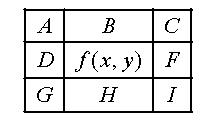
\includegraphics[scale=1.0]{08_segmentace/images/img_8_4.pdf}
    \end{center}
    \caption{Značení hodnot obrazové funkce pro operátor Prewwitové.}
    \label{img:8_4}
\end{figure}

Uvedený postup stanovení derivací průměrem přispívá k redukci šumu. V případech, kdy nezáleží na absolutní velikosti hrany, lze koeficienty 1/3 vypustit. Jestliže po výpočtu velikosti hrany následuje prahování, v~němž se rozhoduje, zda v daném bodě hrana existuje či nikoli, lze vypuštění koeficientů kompenzovat volbou velikosti prahu.

\paragraph{Sobelův operátor:} Tento operátor je podobný operátoru Prewittové. Rozdíl spočívá v tom, že se pro výpočet derivací v jednotlivých směrech používá vážený průměr dle vztahů

\begin{equation} \label{eq:8_10}
    f_{x} \left(x,y\right)=\frac{1}{4} \left[\left(C-A\right)+2\left(F-D\right)+\left(I-G\right)\right],  f_{y} \left(x,y\right)=\frac{1}{4} \left[\left(A-G\right)+2\left(B-H\right)+\left(C-I\right)\right].  
\end{equation} 

I v tomto případě lze za stejných okolností jako u operátoru Prewittové koeficienty 1/4 vypustit.

\paragraph{Kirschův operátor:} Také tento operátor lze zařadit mezi operátory založené na výpočtu gradientu. Veličina mající povahu derivace je počítána celkem v osmi směrech a za velikost hrany je vzata její maximální hodnota. Pro stručnost přeznačíme funkční hodnoty obrazové funkce tak, jak je uvedeno na obr. \ref{img:8_5}. Velikost hrany v bodě ($x$, $y$) se vypočítá dle vzorce

\begin{equation} \label{eq:8_11}
    e\left(x,y\right)=\max\limits_{i=0}^{7} [|5S_{i} - 3T_{i} |],  
\end{equation}
kde
\begin{equation} \label{eq:8_12}
    S_{i} = A_{i} + A_{i+1} + A_{i+2},
\end{equation}

\begin{equation} \label{eq:8_13}
    T_{i} = A_{i+3} + A_{i+4} + A_{i+5} + A_{i+6} + A_{i+7}.
\end{equation}

\begin{figure}[th]
    \begin{center}
        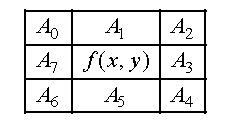
\includegraphics[scale=1.0]{08_segmentace/images/img_8_5.pdf}
    \end{center}
    \caption{Značení hodnot obrazové funkce pro Kirschův operátor.}
    \label{img:8_5}
\end{figure}

Index \textit{i}, pro který je ve výrazu \eqref{eq:8_11} dosaženo maxima, určuje směr hrany. Jestliže ve výrazech \eqref{eq:8_12}, \eqref{eq:8_13} vyjdou hodnoty indexů větší než 7, upraví se operací modulo 8. 

\subsection*{Detekce hran hledáním průchodu druhé derivace nulou}

Z obr. \ref{img:8_2} je zřejmé, že druhá derivace průběhu jasu ve směru napříč hranou nabývá dvou extrémů opačného znaménka a v místě hrany znaménko mění. Protože směr hrany není zpravidla předem znám, je nutné druhou derivaci počítat přinejmenším ve dvou směrech, např. ve směru souřadných os \textit{x},\textit{y}. K výpočtu lze použít Laplaceova operátoru. Zaveďme označení \textit{f}$_{xx}$(\textit{x},\textit{y}) = $\partial^2$\textit{f}(\textit{x},\textit{y})/$\partial x^2$, \textit{f}$_{yy}$(\textit{x},\textit{y}) = $\partial^2$\textit{f}(\textit{x},\textit{y})/$\partial y^2$. Laplaceův operátor je definován vztahem

\begin{equation} \label{eq:8_14}
    \nabla^2 f(x,y)=f_{xx} (x,y) + f_{yy} (x,y).
\end{equation}

Je-li obrazová funkce diskrétní, použijeme místo derivací diference. Pro body uvnitř obrazu (nikoli v krajních řádcích a sloupcích) můžeme použít symetrických diferenčních vzorců

\begin{equation} \label{eq:8_15}
    f_{xx} (x,y)=f(x-1,y)-2f(x,y)+f(x+1,y),
\end{equation}

\begin{equation} \label{eq:8_16}
    f_{yy} (x,y)=f(x,y-1)-2f(x,y)+f(x,y+1).
\end{equation}

Dosazením vztahů \eqref{eq:8_15}, \eqref{eq:8_16} do \eqref{eq:8_14} dostaneme pro realizaci Laplaceova operátoru předpis

\begin{equation} \label{eq:8_17}
    \nabla^2 f(x,y)=f(x+1,y)+f(x-1,y)+f(x,y+1)+f(x,y-1)-4f(x,y).
\end{equation}

Vztah \eqref{eq:8_17} lze vypočítat pomocí konvoluce obrazové funkce \textit{f}(\textit{x},\textit{y}) s konvoluční maskou uvedenou na obr. \ref{img:8_6}a. V souvislosti s určováním hran pomocí druhé derivace bývá uváděna také maska dle obr. \ref{img:8_6}b, která realizuje výpočet součtu druhých derivací ve čtyřech směrech 0$\circ$, 45$\circ$, 90$\circ$, 135$\circ$. Je zřejmé, že v krajních řádcích a sloupcích obrazu nelze masek z obr. \ref{img:8_6} použít. Pro uvedené případy lze v případě potřeby snadno odvodit speciální masky vyžadující pouze hodnoty uvnitř obrazu. Např. pro výpočet hodnoty Laplaceova operátoru v dolním řádku obrazu snadno odvodíme masku dle obr. \ref{img:8_7}a, pro výpočet hodnoty v levém dolním rohu pak masku uvedenou na obr. \ref{img:8_7}b (ostatní potřebné masky získáme rotací masek zde uvedených). Hrany v obraze nalezneme analýzou výsledku poskytnutého Laplaceovým operátorem. Za hranu považujeme místo, kde mezi dvěma dostatečně velikými a dostatečně blízko položenými extrémy opačného znaménka výsledek poskytnutý operátorem mění znaménko.

\begin{figure}[th]
    \begin{center}
        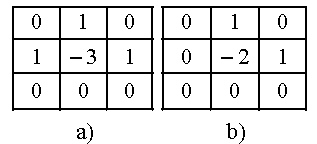
\includegraphics[scale=0.9]{08_segmentace/images/img_8_6.pdf}
    \end{center}
    \caption{Konvoluční masky pro výpočet Laplaceova operátoru..}
    \label{img:8_6}
\end{figure}

\begin{figure}[th]
    \begin{center}
        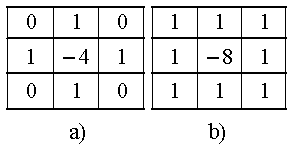
\includegraphics[scale=0.9]{08_segmentace/images/img_8_7.pdf}
    \end{center}
    \caption{Příklady masek pro body na krajích a v rozích obrazu.}
    \label{img:8_7}
\end{figure}

Právě popsaná metoda hledání hran založená na výpočtu druhé derivace a na použití Laplaceova operátoru je dosti citlivá na šum. I při malém zašumění obrazu je detekováno značné množství falešných hran. Problém lze řešit filtrací šumu, která se provede ještě před tím, než jsou hledány hrany. Marr a Hildreth (Maar 80) popsali metodu, v níž pro redukci šumu používají konvoluci s gaussiánem. Protože se tato metoda používá dosti často, popíšeme ji podrobněji. Dvourozměrný gaussián je definován vztahem (obr. \ref{img:8_8})


\begin{equation} \label{eq:8_18}
    G(x, y) = G(x)G(y) = \frac{1}{2\pi \sigma^2} \exp \left( - \frac{x^2 + y^2}{2\sigma^2} \right).
\end{equation}

Hodnotou $\sigma$ lze „regulovat šířku`` gaussiánu a tudíž i míru filtrace. Běžně používané hodnoty $\sigma$ jsou 0.5 až 3. Realizaci konvoluce obrazové funkce s gaussiánem a následnou aplikaci Laplaceova operátoru popisuje vztah

\begin{eqnarray} \label{eq:8_19}
    &\nabla^2& [G(x, y) \ast f(x, y) ] \\
    &=& \left( \frac{\partial^2}{\partial x^2} + \frac{\partial^2}{\partial y^2} \right) \int \int\limits_{-\infty}^{\infty} G(x - \xi, y - \eta) f(\xi, \eta)\,d\xi\,d\eta \nonumber \\
    &=& \left[ \left( \frac{\partial^2}{\partial x^2} + \frac{\partial^2}{\partial y^2} \right) G(x, y) \right] \ast f(x, y) = \left[ \nabla^2 G(x, y) \right] \ast f(x, y).\nonumber
\end{eqnarray}

\begin{figure}[th]
    \begin{center}
        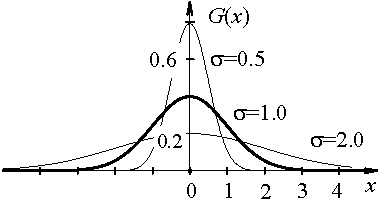
\includegraphics[scale=0.9]{08_segmentace/images/img_8_8.pdf}
    \end{center}
    \caption{Průběh Gaussiánu $G(x)$ pro $\sigma = 0.5$, $\sigma = 1$, $\sigma = 2$.}
    \label{img:8_8}
\end{figure}

Vztah \eqref{eq:8_19} ukazuje, že popisovanou posloupnost akcí lze realizovat konvolucí obrazové funkce s funkcí $\nabla^2 G$. Položíme-li \textit{r} = $\surd(x^2 + y^2)$, můžeme funkci $\nabla^2 G$ zapsat ve tvaru

\begin{equation} \label{eq:8_20}
    \nabla^2 G(r) = \left( \frac{r^2 -2\sigma^2}{2\pi\sigma^6} \right) \exp \left( \frac{-r^2}{2\sigma^2} \right).
\end{equation}

\begin{figure}[th]
    \begin{center}
        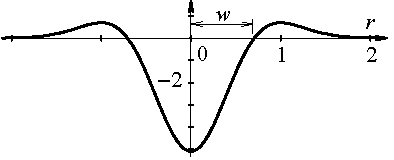
\includegraphics[scale=0.9]{08_segmentace/images/img_8_9.pdf}
    \end{center}
    \caption{Průběh funkce $\nabla^2 G(r)$, $\sigma = 0.5$.}
    \label{img:8_9}
\end{figure}

Funkce $\nabla^2 G$ je rotačně symetrická. Její průběh (průřez průběhu) je znázorněn na obr. \ref{img:8_9}. Označme \textit{w} poloměr kružnice, kde funkce přechází ze záporných do kladných hodnot (obr. \ref{img:8_9}). Z rovnice \eqref{eq:8_20} vychází $w=\sigma\surd 2$. K důkladnějšímu osvětlení principu činnosti této metody vyšetříme ještě frekvenční charakteristiku operátoru $\nabla^2 G$. Provedením Fourierovy transformace a položením \textit{u}$^2$+\textit{v}$^2$ = $\omega^2$ dostaneme

\begin{equation} \label{eq:8_21}
    \mathscr{F} \left\{ \nabla^2 G(x, y) \right\} = \omega^2 \exp \left( - \sigma^2 \frac{\omega^2}{2} \right).
\end{equation}

\begin{figure}[th]
    \begin{center}
        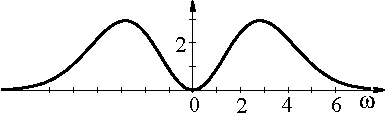
\includegraphics[scale=0.9]{08_segmentace/images/img_8_10.pdf}
    \end{center}
    \caption{Frekvenční charakteristika $\mathscr{F}\{\nabla^2 G\}$ pro $\sigma = 0.5$.}
    \label{img:8_10}
\end{figure}

Průběh frekvenční charakteristiky $\mathscr{F}\{\nabla^2 G\}$ je znázorněn na obr. \ref{img:8_10}. Je zřejmé, že se jedná o pásmový filtr. Vrchol frekvenční charakteristiky vychází v místě $\omega = \surd 2 / \sigma$. Po provedení konvoluce $[\nabla^2 G(x, y)] \ast f(x, y)$ pokračuje metoda hledáním průchodů nulou stejně, jak již bylo popsáno dříve.

\subsection*{Parametrické modely hrany}

Řekněme, že máme rozhodnout, zda je v~obraze v místě o souřadnicích (\textit{x},\textit{y}) hrana. V~pozitivním případě máme stanovit také její velikost a směr. Můžeme to provést tak, že jistým počtem funkčních hodnot obrazové funkce \textit{f}(\textit{x},\textit{y}) z~okolí bodu (\textit{x},\textit{y}) proložíme vhodnou plochu, která průběh obrazové funkce aproximuje. O existenci hrany pak rozhodneme a její parametry stanovíme na základě vyšetřování průběhu aproximující funkce. Aby se potlačil vliv šumu, prokládá se aproximační funkce zpravidla větším počtem funkčních hodnot obrazové funkce, než je nejnižší teoreticky nutný počet. Proložení lze realizovat minimalizací součtu čtverců diferencí funkčních hodnot aproximační funkce od funkčních hodnot obrazové funkce ve zvolených bodech. Nejjednodušší plochou, kterou lze jako modelu hrany použít, je rovina \textit{z} = \textit{ax} + \textit{by} + \textit{c}. Nalezneme-li rovinu aproximující průběh obrazové funkce v~daném místě, pak snadno získáme velikost hrany \textit{e}(\textit{x},\textit{y}) = \textbar grad( \textit{ax} + \textit{by} + \textit{c} )\textbar  = $\surd$(\textit{a}$^2$ + \textit{b}$^2$ ) a také její směr $\varphi$(\textit{x},\textit{y}) = arctg(\textit{b}/\textit{a}) + $\pi$/2. Rovinu můžeme nalézt např. tak, aby co nejlépe aproximovala průběh obrazové funkce ve čtyřech bodech\textit{ f}(\textit{x},\textit{y}), \textit{f}(\textit{x}+1,\textit{y}), \textit{f}(\textit{x},\textit{y}+1) a \textit{f}(\textit{x}+1,\textit{y}+1). Neznámé hodnoty \textit{a},\textit{b},\textit{c} nalezneme minimalizací chyby $\epsilon$ = [\textit{ax} + \textit{by} + \textit{c} $-$ \textit{f}(\textit{x},\textit{y})]$^2$ + [\textit{a}(\textit{x}+1) + \textit{by} + \textit{c} $-$ \textit{f}(\textit{x}+1,\textit{y})]$^2$ + [\textit{ax} + \textit{b}(\textit{y}+1) + \textit{c} $-$ \textit{f}(\textit{x},\textit{y}+1)]$^2$ + [\textit{a}(\textit{x}+1) + \textit{b}(\textit{y}+1) + \textit{c} $-$ \textit{f}(\textit{x}+1,\textit{y}+1)]$^2$ uplatněním podmínek $\partial \epsilon / \partial a = 0$, $\partial$$\epsilon$/$\partial$\textit{b} = 0, $\partial$$\epsilon$/$\partial$\textit{c} = 0.

Dále ukážeme případ, kdy je jako model hrany použita důmyslnější plocha. Předpokládejme např., že v řezu napříč hranou má jas průběh, který je dobře vystižen funkcí

\begin{equation} \label{eq:8_22}
    B + ( A - B ) \Phi(\xi, \sigma).
\end{equation}

Význam parametrů \textit{A},\textit{B} objasňuje obr. \ref{img:8_11}. Funkce $\Phi(\xi, \sigma)$ je integrálem gaussiánu. Je tedy

\begin{equation} \label{eq:8_23}
    \Phi(\xi, \sigma) = \int\limits_{t=-\infty}^{\xi} G(t, \sigma)\,dt, \quad \mathrm{kde} \quad G(t, \sigma) = \exp \left( - \frac{t^2}{2\sigma^2} \right).
\end{equation}

\begin{figure}[th]
    \begin{center}
        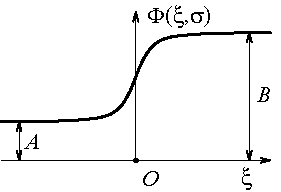
\includegraphics[scale=0.9]{08_segmentace/images/img_8_11.pdf}
    \end{center}
    \caption{Parametrický model hrany.}
    \label{img:8_11}
\end{figure}

\begin{figure}[th]
    \begin{center}
        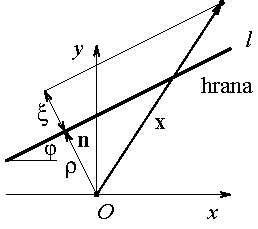
\includegraphics[scale=0.9]{08_segmentace/images/img_8_12.pdf}
    \end{center}
    \caption{Parametrický model hrany (pohled shora).}
    \label{img:8_12}
\end{figure}

Abychom přešli k dvojrozměrnému případu, uvažme, že \textbf{nx} = $\rho$, kde \textbf{n} = ($-$sin $\varphi$, cos $\varphi$), \textbf{x }= (\textit{x},\textit{y}), je rovnice přímky \textit{l} (obr. \ref{img:8_12}). Jestliže bod reprezentovaný vektorem \textbf{x} na přímce \textit{l} neleží, pak vzdálenost bodu od přímky je $\xi$ = \textbf{nx} $-$ $\rho$ = $-$\textit{x} sin $\varphi$ \textit{+} \textit{y} cos $\varphi$ $-$ $\rho$. Předpokládáme-li, že hrana leží na přímce \textit{l}, pak lze průběh jasu v okolí bodu hrany dobře aproximovat funkcí

\begin{equation} \label{eq:8_24}
    B + (A - B) \Phi( - x \sin \varphi + y \cos \varphi - \rho, \sigma).
\end{equation}

Celkem má tedy popsaný model pět parametrů \textit{A},\textit{B},$\sigma$,$\varphi$,$\rho$. Hodnota (\textit{A}$-$\textit{B}) určuje velikost (výšku) hrany, parametr $\sigma$ její strmost a parametr $\varphi$ směr hrany v bodě \textbf{x}. Parametry lze určit na základě podmínky, aby se v jistému počtu bodů (pixelů) ležících v okolí bodu \textbf{x} hodnoty funkce \eqref{eq:8_24} co nejvíce přimykaly skutečným hodnotám obrazové funkce. Nejmenší počet bodů umožňující úlohu řešit je pět. S ohledem na redukci šumu je však výhodnější volit počet bodů vyšší. Pro hledané parametry lze pak sestavit předeterminovaný systém, který je možné řešit minimalizací chyby. Jistou komplikací ovšem je, že se jedná o problém nelineární. K jeho řešení je proto zapotřebí použít numerických metod.

\subsection*{Cannyho detektor hran}

Popisovaný detektor hran byl publikován Cannym (Canny 83, 86) a později detailně studován mnoha dalšími autory. Při návrhu detektoru vycházel Canny z~toho, že starší detektory hran byly konstruovány více či méně intuitivně, a formuloval proto požadavky, které by měl detektor splňovat. K~nalezení detektoru pak přistoupil jako k~optimalizační úloze (tj. hledal detektor, který vytyčené požadavky splňuje co nejlépe). Cannym navržené požadavky byly následující: 1) minimalizovat pravděpodobnost chybné detekce, 2) najít polohu hrany v obraze co nejpřesněji, 3) bod hrany identifikovat jednoznačně. Postup, který vede k~návrhu odpovídajícího filtru, popíšeme podrobněji.

Předpokládejme nejprve, že vstupní signál je jednorozměrný (získané výsledky později zobecníme i na signály dvojrozměrné). Matematickým modelem hrany ve vstupním signálu (ve shodě s původním pramenem označíme vstupní signál \textit{I}(\textit{x})) je skok výšky \textit{A} umístěný do počátku. Doplněn je dále aditivní šum \textit{n}(\textit{x}) (obr. \ref{img:8_13}). Předpokládáme, že šum je bílý s~nulovou střední hodnotou. Vstupní signál má tedy tvar

\begin{equation} \label{eq:8_25}
    I(x) = Au_{-1}(x) + n(x), \quad \mathrm{kde} \quad u_{-1}(x) = \left\{ \begin{array}{ccc}
    0 & \mathrm{pro} & x < 0 \\
    1 & \mathrm{pro} & x \geq 0
    \end{array}\right. .
\end{equation}

Předpokládáme, že hranový operátor bude založen na výpočtu konvoluce vstupního signálu s~funkcí \textit{f}(\textit{x}). Tuto funkci, kterou zatím neznáme, stanovíme tak, aby byla co nejlépe splněna kriteria formulovaná v~úvodu této podkapitoly. Označme $O(x_0)$ signál, který je výsledkem konvoluce. Podle definice konvoluce máme

\begin{equation} \label{eq:8_26}
    O(x_0) = \int\limits_{-\infty}^{\infty} I(x_0 - x) f(x)\,dx .
\end{equation}

\begin{figure}[th]
    \begin{center}
        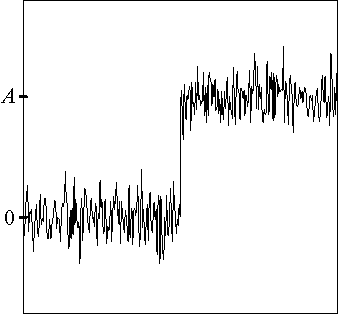
\includegraphics[scale=0.9]{08_segmentace/images/img_8_13.pdf}
    \end{center}
    \caption{Průběh signálu ve směru napříč hranou.}
    \label{img:8_13}
\end{figure}

Nejprve vyhodnotíme, jaký výstup v bodě \textit{x}$_0$ = 0 odpovídá skoku velikosti \textit{A} (bez šumu). Dosazením rovnice \eqref{eq:8_25} do rovnice \eqref{eq:8_26} a položením \textit{n}(\textit{x}) = 0, \textit{x}$_0$ = 0 dostaneme

\begin{equation} \label{eq:8_27}
    \int\limits_{-\infty}^{\infty} Au_{-1}(-x)f(x)\,dx = A \int\limits_{-\infty}^{0} f(x)\,dx .
\end{equation}

Dále vypočítáme střední hodnotu čtverce signálu, který na svém výstupu poskytuje operátor v bodě \textit{x}$_0$ = 0, jestliže je na vstup přiložen pouze šum \textit{n}(\textit{x}). Dostaneme 

\begin{equation} \label{eq:8_28}
    \mathrm{E} \left\{ \left[ \int\limits_{-\infty}^{\infty} n(-x)f(x)\,dx \right]^2 \right\} = \int\limits_{-\infty}^{\infty} \mathrm{E} \left\{ n^2(-x) \right\} f^2(x)\,dx = n_0^2 \int\limits_{-\infty}^{\infty} f^2(x)\,dx .
\end{equation}

Při úpravě výše uvedeného vztahu jsme se opírali o předpoklad, že \textit{n}(\textit{x}) je bílý šum s~nulovou střední hodnotou a že tedy pro všechna \textit{x}$_1$ $\neq$ \textit{x}$_2$ platí E\{\textit{n}(\textit{x}$_1$)\textit{n}(\textit{x}$_2$)\} = 0. Dále jsme předpokládali, že hodnota E\{\textit{n}$^2$(\textit{x})\} je pro všechna \textit{x} konstatní, a položili jsme proto E\{\textit{n}$^2$(\textit{x})\} = \textit{n}$_0^2$ (jedná se o varianci šumové složky vstupního signálu). Definujme poměr signál/šum (\textit{SNR}) jako podíl odezvy na skok velikosti \textit{A} ku odmocnině střední hodnoty čtverce odezvy na šum. Pro hodnocení pravděpodobnosti chybné detekce dále zaveďme míru $\Sigma$ \textit{=} \textit{n}$_0$\textit{ SNR / A}, která je závislá pouze na hledané funkci \textit{f}(\textit{x}), nikoli na velikosti vstupního signálu. Máme tedy

\begin{equation} \label{eq:8_29}
    SNR = \frac{\int\limits_{-\infty}^{0} f(x)\,dx}{n_0 \sqrt{\int\limits_{-\infty}^{\infty} f^2(x)\,dx}}, \quad \sum = \frac{n_0}{A} SNR = \frac{\int\limits_{-\infty}^{0} f(x)\,dx}{\sqrt{\int\limits_{-\infty}^{\infty}f^2(x)\,dx}} .
\end{equation}

Při detekci hrany právě konstruovaným hranovým operátorem budeme za hranu považovat místo, kde operátor (konvoluce s \textit{f}) dává největší hodnotu. V případě hrany umístěné do počátku by to teoreticky mělo být místo \textit{x}$_0$ = 0. Šum však způsobí, že tomu tak nebude zcela přesně. Nalezneme proto místo, kde výstup operátoru nabývá extrému. K~tomu vypočítáme první derivaci výstupního signálu a položíme ji rovnu nule

\begin{equation} \label{eq:8_30}
    \frac{d}{dx_0} O(x_0) = O'(x_0) = \frac{d}{dx_0} \int\limits_{-\infty}^{\infty} I(x_0 - x) f(x_0 - x)\,dx.
\end{equation}

Pro derivování konvoluce máme

\begin{eqnarray} \label{eq:8_31}
    \frac{d}{dx_0} \int\limits_{-\infty}^{\infty} I(x_0 - x) f(x)\,dx &=& \frac{d}{dx_0} \int\limits_{-\infty}^{\infty} I(x)f(x_0 - x)\,dx \\
    &=& \int\limits_{-\infty}^{\infty} I(x) f'(x_0 - x)\,dx = \int\limits_{-\infty}^{\infty} I(x_0 - x) f'(x)\,dx .\nonumber
\end{eqnarray}

Výstup rozdělíme na složku odpovídající skoku umístěnému do počátku a na složku odpovídající šumu. Tyto složky označíme postupně \textit{O}$_n$, \textit{O}$_n$. Derivace odezvy na skok má v bodě \textit{x}$_0$ velikost

\begin{equation} \label{eq:8_32}
    O_s'(x_0) = \int\limits_{-\infty}^{\infty} Au_{-1}(x_0 - x) f'(x)\,dx = A \int\limits_{-\infty}^{x_0} f'(x)\,dx = A f(x_0).
\end{equation}

Derivaci \textit{O'}$_s$(\textit{x}$_0$) odezvy na skok rozvineme kolem počátku v Taylorovu řadu. Předpokládáme při tom, že hledaná funkce \textit{f}(\textit{x}) bude antisymetrická, a že proto bude platit \textit{f}(0) = 0. Dostaneme

\begin{equation} \label{eq:8_33}
    O_s'(x_0) = Af(x_0) = Af(0) + x_0 Af'(0) = x_0Af'(0).
\end{equation}

Derivací odezvy hranového operátoru na šum bude náhodná proměnná s nulovou střední hodnotou a s variancí

\begin{equation} \label{eq:8_34}
    \mathrm{E} \left\{ O_n'^2(x_0) \right\} = \mathrm{E} \left\{ \left[ \int\limits_{-\infty}^{\infty} n(x_0 - x) f'(x)\,dx \right]^2 \right\} = n_0^2 \int\limits_{-\infty}^{\infty} f'^2(x)\,dx.
\end{equation}

Pro podmínku extrému pak máme

\begin{equation} \label{eq:8_35}
    O_s'(x_0) = O_s'(x_0) + O_s'(x_0) = 0 \quad \mathrm{a tedy} \quad O_s'(x_0) = -O_n'(x_0).
\end{equation}

Z předchozí rovnice dále plyne

\begin{equation} \label{eq:8_36}
    \mathrm{E} \left\{ O_s'^2(x_0) \right\} = \mathrm{E} \left\{ O_n'^2(x_0) + O_s'(x_0) \right\}.
\end{equation}

Dosazením vztahů \eqref{eq:8_33} a \eqref{eq:8_34} do rovnice \eqref{eq:8_36} dostaneme:

\begin{equation} \label{eq:8_37}
    \mathrm{E} \left\{ x_0^2 \right\} = \frac{n_0^2 \int\limits_{-\infty}^{\infty} f'^2(x)\,dx}{A^2 f'^2(0)} = \sigma_{x_0}^2.
\end{equation}

V předchozím výraze jsme označení $\sigma$\textit{x}$_0$ použili pro aproximaci směrodatné odchylky polohy maxima na výstupu operátoru od skutečné polohy skoku, který leží v počátku. Schopnost operátoru správně lokalizovat hranu hodnotíme podle převrácené hodnoty této odchylky. Zavedeme míru $\Lambda = n_0/(\sigma_{x_0} A)$, která závisí pouze na vlastnostech hranového operátoru a nikoli na signálu. S využitím vztahu \eqref{eq:8_37} dostaneme

\begin{equation} \label{eq:8_38}
    \Lambda = \frac{|f'(0)|}{\sqrt{\int\limits_{-\infty}^{\infty} f'^2(x)\,dx}} .
\end{equation}

Výkonnost hranového operátoru pak hodnotíme součinem $\Sigma\Lambda$. S využitím vztahů \eqref{eq:8_29}, \eqref{eq:8_38} máme

\begin{equation} \label{eq:8_39}
    \sum(f)\Lambda(f) = \frac{\int\limits_{-\infty}^{0} f(x)\,dx}{\sqrt{\int\limits_{-\infty}^{\infty} f^2(x)\,dx}} \frac{|f'(0)|}{\sqrt{\int\limits_{-\infty}^{\infty} f'^2(x)\,dx}} .
\end{equation}

Poslední podmínkou je, aby jedné hraně odpovídalo pokud možno jediné maximum na výstupu operátoru. Tento požadavek vyjádříme jako požadavek na funkci \textit{f}(\textit{x}). Využijeme pomocného tvrzení, které uvedeme bez důkazu a které říká, že střední vzdálenost \textit{x}$_{zc}$ mezi dvěma průchody nulou odezvy funkce \textit{g} na gaussovský šum je dána výrazem (odezvou se rozumí konvoluce funkce \textit{g} s šumem) 

\begin{equation} \label{eq:8_40}
    x_{zc} = \pi \left( \frac{-R(0)}{R''(0)} \right)^{\frac{1}{2}},
\end{equation}
kde \textit{R}($\tau$) je autokorelační funkce funkce \textit{g}. Snadno ověříme, že platí (předpokládáme \textit{g}($-$$\infty$)= \textit{g}($\infty$) = 0)

\begin{equation} \label{eq:8_41}
    R(0) = \int\limits_{-\infty}^{\infty} g^2(x)\,dx, \quad R''(0) = \int\limits_{-\infty}^{\infty} g(x) g''(x)\,dx = - \int\limits_{-\infty}^{\infty} g'^2(x)\,dx .
\end{equation}

V našem případě hledáme střední vzdálenost \textit{x}$_{zc}$ mezi dvěma průchody nulou odezvy funkce \textit{f'} . Ze vztahů \eqref{eq:8_40}, \eqref{eq:8_41} dostaneme

\begin{equation} \label{eq:8_42}
    x_{zc} = \pi \left( \frac{\int\limits_{-\infty}^{\infty} f'^2(x)\,dx}{\int\limits_{-\infty}^{\infty} f''^2(x)\,dx} \right)^{\frac{1}{2}}.
\end{equation}

Vzdálenost \textit{x}$_{\max}$ mezi dvěma přilehlými maximy odezvy funkce na šum je dvojnásobkem \textit{x}$_{zc}$. Tuto hodnotu vyjádříme relativně vzhledem k šířce operátoru. Šířkou operátoru rozumíme interval $\langle-W, W\rangle$. Na tomto intervalu předpokládáme funkční hodnoty \textit{f} nenulové (mimo tento interval předpokládáme funkční hodnoty nulové; dále připomeňme, že funkci \textit{f} předpokládáme antisymetrickou). Je tedy

\begin{equation} \label{eq:8_43}
    x_{\max} = 2 x_{zc} = kW.
\end{equation}

Schopnost detektoru identifikovat hranu jednoznačně bude tím lepší, čím vyšší bude hodnota \textit{k}. Dosud neznámá funkce \textit{f} by tedy měla maximalizovat výraz \eqref{eq:8_39} a při tom dávat pokud možno co nejvyšší hodnotu \textit{k}. V (Canny 83) je popsáno řešení založené na maximalizaci funkcionálu \eqref{eq:8_39}. Jsou postupně voleny různé hodnoty \textit{k} (0.075 až 0.7) a rovnice \eqref{eq:8_43} je použita jako doplňující podmínka. Pro každou hodnotu \textit{k} je numerickou optimalizací stanovena funkce \textit{f}. Na základě takto získaných výsledků je ukázáno, že pro vyšší hodnoty \textit{k} (což je prakticky zajímavý případ) lze hledanou funkci \textit{f} dosti dobře aproximovat pomocí první derivace gaussiánu. Na tuto možnost se dále zaměříme. Připomeňme, že gaussián je definován předpisem

\begin{equation} \label{eq:8_44}
    G(x) = \exp \left( - \frac{x^2}{2\sigma^2} \right).
\end{equation}

Funkce \textit{f} má tedy tvar

\begin{equation} \label{eq:8_45}
    f(x) \approx G'(x) = -\frac{x}{\sigma^2} \exp \left( - \frac{x^2}{2\sigma^2} \right).
\end{equation}

Pro výše uvedenou aproximaci funkce \textit{f} vypočteme následující hodnoty (Canny 83)

\begin{equation} \label{eq:8_46}
    |f'(0)| = \frac{1}{\sigma^2}, \; \int\limits_{-\infty}^{0} f(x)\,dx = 1, \; \int\limits_{-\infty}^{\infty} f^2(x)\,dx = \frac{\sqrt{x}}{2\sigma},
\end{equation}

\begin{equation}
    \int\limits_{-\infty}^{\infty} f'^2(x)\,dx = \frac{3\sqrt{\pi}}{4\sigma^3}, \; \int\limits_{-\infty}^{\infty} f''^2(x)\,dx = \frac{15\sqrt{\pi}}{8\sigma^5}.\nonumber
\end{equation}

Odtud pak index $\Sigma\Lambda$ výkonnosti operátoru a hodnota \textit{k} pro operátor \textit{f}(\textit{x}) = \textit{G}'(\textit{x}) vychází

\begin{equation} \label{eq:8_47}
    \Sigma\Lambda = \sqrt{\frac{8}{3\pi}} = 0.92 \quad \mathrm{a} \quad k = \sqrt{\frac{4}{15}} = 0.51.
\end{equation}

Zjištěné hodnoty jsou jen o málo menší než hodnoty pro operátor optimální. Podstatnou výhodou použití gaussiánu je ale snadný výpočet.

Až doposud jsme se soustředili na jednorozměrný případ. Zbývá ukázat, jak pracuje Cannyho detektor v případě dvojrozměrném. Předpokládejme nejprve, že máme hledat hrany známého směru. Ve směru napříč hranou použijeme konvoluci s právě nalezenou funkcí \textit{f}. Ve směru podél hrany uplatníme projekci. Jestliže je \textit{f}  aproximována derivací gaussiánu, pak je výhodné, aby funkcí realizující projekci byl rovněž gaussián (projekce bude počítána jako konvoluce s gaussiánem). Jako obvykle není zapotřebí výpočet provádět pro všechny možné směry hran, ale postačí jej provést pro dva směry (např. \textit{x},\textit{y}). Nechť \textit{I}(\textit{x},\textit{y}) je obrazová funkce. Pro hrany rovnoběžné s osou \textit{y} a hrany rovnoběžné s osou \textit{x} pak dává hranový operátor následující hodnoty

\begin{equation} \label{eq:8_48}
    [ I(x, y) \ast G(y)] \ast G_x(x) = \frac{\partial}{\partial x} \left\{ I(x, y) \ast \left[ G(x)G(y) \right] \right\} = E_x(x, y),
\end{equation}

\begin{equation} \label{eq:8_49}
    [ I(x, y) \ast G(x)] \ast G_y(y) = \frac{\partial}{\partial y} \left\{ I(x, y) \ast \left[ G(x)G(y) \right] \right\} = E_y(x, y).
\end{equation}

V uvedených výrazech realizuje první člen v hranatých závorkách projekci. Výstupem dvojrozměrného detektoru hran je vektorové pole \textbf{E}(\textit{x},\textit{y}) = (\textit{E}$_x$(\textit{x},\textit{y}), \textit{E}$_y$(\textit{x},\textit{y})). Pro velikost a směr hrany máme

\begin{equation} \label{eq:8_50}
    |\mathbf{E}(x, y)| = \sqrt{E_x^2(x, y) + E_y^2(x, y)}, \; \varphi(x, y) = \arctan(E_y(x, y) / E_x(x, y)) + \pi / 2.
\end{equation}

Řekneme, že v nějakém bodě obrazu je hrana, jestliže \textbar \textbf{E}(\textit{x},\textit{y})\textbar  v tom bodě nabývá lokálního extrému (připomeňme, že jsme se snažili, aby jedné hraně příslušelo pouze jediné maximum) a jestliže je hodnota \textbar \textbf{E}(\textit{x},\textit{y})\textbar  v tom bodě dostatečně veliká. Předpokládejme nyní, že je obraz popsán diskrétní obrazovou funkcí. Zaměřme se nejdříve na první podmínku. Bod (\textit{x},\textit{y}) může být bodem hrany jen tehdy, jestliže platí (obr. \ref{img:8_14})

\begin{equation} \label{eq:8_51}
    |\mathbf{E}_{-\theta}| < |\mathbf{E}(x, y)| > |\mathbf{E}_{+\theta}|
\end{equation}

Hodnoty \textbar \textbf{E}$_{+\theta}$\textbar, \textbar \textbf{E}$_{-\theta}$\textbar stanovíme interpolací (obr. \ref{img:8_14}). Např. leží-li směr gradientu v prvním oktantu, pak máme

\begin{equation} \label{eq:8_52}
    |\mathbf{E}_{+\theta}| = \alpha |\mathbf{E}(x+1, y+1)| + (1 - \alpha) |\mathbf{E}(x+1, y)|,
\end{equation}

\begin{equation} \label{eq:8_53}
    |\mathbf{E}_{-\theta}| = \alpha |\mathbf{E}(x-1, y-1)| + (1 - \alpha) |\mathbf{E}(x-1, y)|.
\end{equation}

\begin{figure}[th]
    \begin{center}
        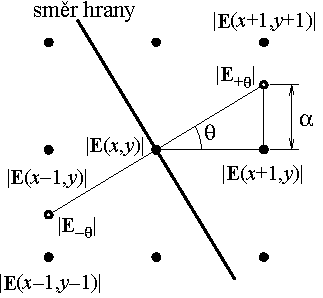
\includegraphics[scale=0.9]{08_segmentace/images/img_8_14.pdf}
    \end{center}
    \caption{K rozhodnutí maxima.}
    \label{img:8_14}
\end{figure}

Význam hodnoty $\alpha$ je patrný z obr. \ref{img:8_14}. Podobné vztahy lze snadno odvodit i pro zbývající oktanty. Podmínku, že hodnota \textbar \textbf{E}(\textit{x},\textit{y})\textbar  má být v bodě hrany dostatečně velká, lze realizovat prahováním. Účinné je prahování s hysterezí, při němž se používá dvou hodnot prahu $t_{\mathrm{low}}$, $t_{\mathrm{high}}$. Za body hrany jsou nejprve označeny všechny pixely, kde je velikost hrany větší než $t_{\mathrm{high}}$. Dále jsou pak za body hrany označeny také ty pixely, kde je velikost hrany větší než $t_{\mathrm{low}}$ (ale menší než $t_{\mathrm{high}}$) a které sousedí s pixelem, který byl již dříve označen za bod hrany. Tento krok lze opakovat několikrát.

%\noindent \textbf{8.1.5  Stanovení hran na základě textury}

%\noindent V tomto odstavci se zaměříme na detekci hran tvořených náhlou změnou textury ve vyšetřovaném obraze. Jednoduché je řešení, které předpokládá, že v důsledku rozdílnosti textur po obou stranách hrany je rozdílná také střední hodnota jasu v oblastech přiléhajících k hraně. Nechť \textit{f} (\textit{r})(\textit{x},\textit{y}) označuje střední hodnotu jasu v kruhovém okolí bodu (\textit{x},\textit{y}). Poloměr okolí je \textit{r}. Předpokládejme, že v obraze máme hranu, jejíž směr je $\varphi$ + $\pi$/2. Umístěme dvě taková okolí \textit{f} (\textit{r})(\textit{xL},\textit{yL}), \textit{f} (\textit{r})(\textit{xR},\textit{yR}) nalevo a napravo od hrany (obr.8.15) a určeme diferenci 

% \textit{f}$\varphi$(\textit{r})(\textit{x},\textit{y}) = $\mid$ \textit{f} (\textit{r})(x\textit{R},y\textit{R}) $-$ \textit{f} (\textit{r})(\textit{xL},\textit{yL}) $\mid$ \eqref{GrindEQ__8_54_}

%  = $\mid$ \textit{f} (\textit{r})(\textit{x} + \textit{r} cos$\varphi$, \textit{y} + \textit{r} sin$\varphi$) $-$ \textit{f} (\textit{r})(\textit{x} $-$ \textit{r} cos$\varphi$, \textit{y} $-$ \textit{r} sin$\varphi$) $\mid$.

%\noindent Existence hrany v bodě (\textit{x},\textit{y}) se projeví vysokými hodnotami \textit{f}$\varphi$(\textit{r})(\textit{x},\textit{y}). Výraz \eqref{GrindEQ__8_54_} předpokládá znalost směru hrany. Není-li směr znám, lze vypočítat diference ve směru os \textit{x} a \textit{y}, kterých pak použijeme stejně, jak bylo popsáno u metody gradientní. Pro diference a velikost hrany máme

% ,   , \eqref{GrindEQ__8_55_}

% . \eqref{GrindEQ__8_56_}

%\noindent Při praktické realizaci je možné nahradit kruhové okolí bodu (\textit{x},\textit{y}) praktičtějším okolím čtvercovým, pro které lze střední hodnotu obrazové funkce vyjádřit jednoduše vztahem

% . \eqref{GrindEQ__8_57_}

%\noindent 

%\noindent Volba poloměru okolí \textit{r} zaslouží pozornosti. Jestliže je poloměr příliš malý, pak není v procesu průměrování dostatečně vyhlazen vzorek textury, což způsobuje detekci falešných hran. Příliš velký poloměr naopak způsobí, že nejsou detekovány krátké hrany. Je proto výhodné stanovit poloměr okolí na základě velikosti nejmenšího objektu, který má být detekován. Volbu je zpravidla nutné ověřit experimentem. Naznačme na závěr ještě jeden poněkud komplikovanější postup pro detekci hran z textury. Uvažujme bod (\textit{x},\textit{y}) a jeho dvě okolí tak, jak bylo naznačeno na obr. 8.15. Pro obě okolí sestrojíme normalizované histogramy \textit{pL}(\textit{z}), \textit{pR}(\textit{z}) jasů. Usuzujeme, že rozdílné histogramy implikují existenci hrany v bodě (\textit{x},\textit{y}). Míru rozdílnosti obou histogramů lze určit např. ze vztahu .

%\noindent 

%\noindent \textbf{8.1.6 Hledání hran v barevných obrazech}

%\noindent Až doposud jsme předpokládali, že zpracovávaný obraz je v každém místě charakterizován jedinou skalární hodnotou - úrovní jasu. Máme-li hledat hrany v barevných obrazech, můžeme je před zpracováním převést na černobílé a dále je zpracovávat dříve popsanými postupy. Nevýhodou tohoto přístupu je ovšem ztráta jisté části informace. Proto může být někdy výhodné zpracovávat barevné obrazy přímo, bez jejich převodu na obrazy černobílé. Předpokládejme, že barva každého bodu obrazu je popsána trojicí \textit{r},\textit{g},\textit{b} intenzit červené, zelené a modré barevné složky. Barevný obraz je tedy popsán vektorovou obrazovou funkcí
%\begin{equation} \label{GrindEQ__8_58_} 
%f(x,y)=\left(r(x,y),g(x,y),b(x,y)\right).  
%\end{equation} 
%Pro stanovení hran v barevných obrazech můžeme upravit např. již dříve popsanou gradientní metodu. Jako velikost hrany můžeme vzít např. hodnotu
%\begin{equation} \label{GrindEQ__8_59_} 
%e\left(x,y\right)=\sqrt{\left|{\rm grad}\left(r(x,y)\right)\right|^{2} +\left|{\rm grad}\left(g(x,y)\right)\right|^{2} +\left|{\rm grad}\left(b(x,y)\right)\right|^{2} } .  
%\end{equation} 
%Za směr hrany můžeme považovat směr kolmý k vektoru
%\begin{equation} \label{GrindEQ__8_60_} 
%g(x,y)={\rm grad}(r(x,y))+{\rm grad}(g(x,y))+{\rm grad}(b(x,y)).  
%\end{equation} 
%Při praktické realizaci uvedených vztahů opět nahradíme derivace diferencemi. Na závěr poznamenejme, že podle našich zkušeností jsou výsledky získané analýzou barevných obrazů sice jednoznačně lepší než v případě převodu na obraz černobílý, avšak toto zlepšení není vždy tak významné, aby vyvážilo komplikace při výpočtu.

%\noindent 

\section*{Spojování hran}

Hranové operátory z~předchozí podkapitoly určovaly velikost a případně i směr hrany jednotlivě v každém bodě obrazu, tedy lokálně. To je ovšem poněkud v rozporu s intuitivní představou hran jako delších souvislých úseček případně křivek v obrazech. Hrany chápané tímto druhým způsobem nazýváme v této podkapitole globálními hranami. K nalezení globálních hran lze využít výsledků poskytovaných lokálními operátory, které jsou však dále zpracovány v procesu tzv. spojování hran. Proces spojování je ilustrován na obr. \ref{img:8_16}. Ve vyobrazeném případě umožňují lokálně stanovené velikosti a směry hran snadno proložit hranu globální.

\begin{figure}[th]
    \begin{center}
        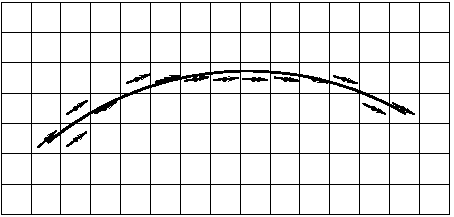
\includegraphics[scale=0.9]{08_segmentace/images/img_8_16.pdf}
    \end{center}
    \caption{Proložení globální hrany.}
    \label{img:8_16}
\end{figure}

%\noindent \textbf{8.2.1 Heuristické sledování hrany}

%\noindent V heuristických metodách sledování hrany jsou globální hrany předpokládány ve tvaru úsečky nebo křivky (často se např. jedná o kruhový oblouk). Vstupní informací pro tyto metody je obraz, v němž je pro každý pixel stanovena velikost a případně i směr hrany. Takový obraz lze získat pomocí některého z lokálních hranových operátorů. Někdy se také může jednat o naskenovaný obraz technického výkresu, v němž jsou čáry po naskenování upraveny ztenčováním. Heuristické sledování globální hrany zahrnuje zpravidla následující kroky: 1) nalezení počátečního bodu globální hrany,  2) predikce polohy následujícího bodu, 3) hledání bodu hrany v okolí predikované polohy, 4) určení následujícího kroku algoritmu. Jednotlivé kroky popíšeme dále podrobněji. 

%\noindent Nalezení počátečního bodu globální hrany: V tomto kroku nalezneme postupným prohledáváním vstupního obrazu některý bod globální hrany. Je nutné, aby tento bod byl detekován spolehlivě, což lze zajistit volbou vysoké hodnoty prahu. Jestliže je k dispozici také směr hrany, lze této informace použít pro predikci polohy druhého bodu hrany. Není-li směr k dispozici, hledáme druhý bod hrany mezi všemi sousedy bodu prvního.

%\noindent Predikce polohy následujícího bodu: Jestliže již bylo nalezeno několik předchozích bodů hrany, pak lze na základě této znalosti a na základě očekávaného tvaru hrany (úsečka, křivka) odhadnout polohu následujícího bodu. Podle očekávaného tvaru globální hrany proložíme doposud nalezenými body přímku nebo křivku. K proložení se často používá metody nejmenších čtverců. Proložením snadno získáme predikci polohy následujícího bodu. Pro stanovení okolí, ve kterém má být následující bod hledán, se používají různé heuristické vztahy, které se opírají o úvahu, že čím více bodů hrany bylo již nalezeno a čím kvalitněji lze předpokládaný tvar nalezenými body proložit, tím je odhad polohy následujícího bodu jistější, a prohledávané okolí může být proto menší. Predikovat lze rovněž očekávanou velikost lokální hrany, což umožňuje stanovit vhodnou velikost prahu, který bude v následujícím bodě pro rozhodnutí o existenci hrany použit.

%\noindent Hledání bodu v okolí predikované polohy: Bod hrany hledáme v oblasti, jejíž poloha a velikost byly  stanoveny predikcí. Jestliže je ve stanoveném okolí nalezeno více vyhovujících bodů, lze vybrat nejlepší z nich (tj. bod, který je blízko predikované polohy a v němž je vysoká velikost hrany). 

%\noindent Určení následujícího kroku: Je nutné rozhodnout, zda lze ve sledování globální hrany pokračovat nebo zda má být sledování ukončeno. Jestliže je ve stanoveném okolí nalezen bod, který dostatečně přesně odpovídá predikci a jestliže lze předpokládaný tvar hrany proložit dosud nalezenou množinou bodů dostatečně kvalitně, lze ve sledování pokračovat. Jinak je nutné sledování ukončit. Kvalitu proložení lze hodnotit např. pomocí maxima vzdálenosti nalezených bodů od prokládané křivky.

%\noindent Po ukončení sledování jedné hrany přechází algoritmus na sledování hrany následující. Hrany, které již byly nalezeny, jsou ze vstupního obrazu odstraněny, aby nebyly detekovány opakovaně. Metody heuristického sledování hrany jsou účinné. Jejich implementace je však bohužel obtížnější a vyžaduje pracné řešení řady drobných detailů.

%\noindent 

%\noindent 

%\noindent Na závěr tohoto odstavce poznamenejme, že jednou z možností, jak popsat extrahované křivky, je použít tzv. Freemanova kódu. Ve Freemanově kódu je křivka popsána od jednoho ze svých konců. Postupně jsou zapisovány kódy směrů tak, jak křivka postupuje od jednoho pixelu k pixelu následujícímu. Kódování směrů ukazuje obr. 8.17. Příklad kódování křivky je uveden na obr. 8.18. Extrahované křivky lze ovšem také popsat pomocí úseček a oblouků (kruhových nebo parabolických), které jimi lze proložit. Někdy je popis pomocí Freemanova kódu mezistupněm k~získání uvedeného  popisu.

%\noindent 

%\noindent \textbf{8.2.2 Proložení přímky a křivky}

%\noindent V tomto odstavci ukážeme, jak lze metodou nejmenších čtverců proložit danou množinou bodů přímku, kružnici nebo kruhový oblouk. Zaměříme se nejprve na přímku. Rovnici přímky uvažujeme ve tvaru $\alpha$\textit{x} + $\beta$\textit{y} + $\gamma$  = 0. Předpokládejme, že $\beta$ $\neq$ 0, a dělme rovnici touto hodnotou. Dostane rovnici \textit{ax} + \textit{y} + \textit{c} = 0. Přímka má být proložena \textit{n} body. Souřadnice \textit{i}-tého bodu označme \textit{xi},\textit{yi}. Hodnota $\epsilon$\textit{i} = \textit{axi} + \textit{yi} + \textit{c} je úměrná vzdálenosti \textit{i}-tého bodu od přímky. Hodnoty \textit{a},\textit{c} lze stanovit z podmínky, aby součet čtverců hodnot $\epsilon$\textit{i} byl minimální. Hledáme tedy minimum výrazu
%\begin{equation} \label{GrindEQ__8_61_} 
%\varepsilon =\sum _{i=1}^{n}\varepsilon _{i}^{2}  =\sum _{i=1}^{n}\left(ax_{i} +y_{i} +c\right)^{2}  .  
%\end{equation} 
%Obvyklým postupem, kdy položíme $\partial$$\epsilon$/$\partial$\textit{a} = 0 a $\partial$$\epsilon$/$\partial$\textit{c} = 0, obdržíme následující výsledek
%\begin{equation} \label{GrindEQ__8_62_} 
%a=\frac{\sum _{i=1}^{n}x_{i}  \sum _{i=1}^{n}y_{i}  -n\sum _{i=1}^{n}x_{i} y_{i}  }{n\sum _{i=1}^{n}x_{i}^{2}  -\left(\sum _{i=1}^{n}x_{i}  \right)^{2} } ,     c=\frac{\sum _{i=1}^{n}x_{i}  \sum _{i=1}^{n}x_{i} y_{i}  -\sum _{i=1}^{n}x_{i}^{2} \sum _{i=1}^{n}y_{i}   }{n\sum _{i=1}^{n}x_{i}^{2}  -\left(\sum _{i=1}^{n}x_{i}  \right)^{2} } .  
%\end{equation} 
%Dosažená hodnota $\epsilon$ určuje kvalitu proložení. Pokud by pro prokládanou přímku platilo $\beta$ = 0, pak nelze provést dělení rovnice přímky hodnotou $\beta$. V takovém případě lze ovšem dělit hodnotou $\alpha$, což dává rovnici \textit{x} + \textit{by} + \textit{c} = 0. Tento případ lze řešit analogicky jako případ předchozí. Výsledné vztahy pro \textit{b},\textit{c} vycházejí podobně - postačí zaměnit \textit{a} za \textit{b} a prohodit \textit{xi} a \textit{yi}. V praxi zpravidla dopředu nevíme, který z obou případů nastane. Můžeme proto vypočítat hodnoty jmenovatele ve vzorcích pro obě varianty a použít tu, pro níž je absolutní hodnota jmenovatele větší. 

%\noindent Při proložení kružnice vyjdeme z rovnice kružnice (\textit{x} $-$ \textit{a})2 + (\textit{y} $-$ \textit{b})2 $-$ \textit{r}2 = 0, kde \textit{a},\textit{b} jsou hledané souřadnice středu kružnice a \textit{r} je její poloměr. Metodou nejmenších čtverců lze snadno odvodit řešení, kdy minimalizujeme součet čtvrtých mocnin vzdáleností zadaných bodů od prokládané kružnice. Minimalizujeme tedy hodnotu
%\begin{equation} \label{GrindEQ__8_63_} 
%\varepsilon =\sum _{i=1}^{n}\left[\left(x_{i} -a\right)^{2} +\left(y_{i} -b\right)^{2} -r^{2} \right]^{2}  .  
%\end{equation} 
%Položíme-li $\partial$$\epsilon$/$\partial$\textit{a} = 0, $\partial$$\epsilon$/$\partial$\textit{b} = 0,  $\partial$$\epsilon$/$\partial$\textit{r} = 0, pak po zdlouhavém výpočtu obdržíme výsledek

% , \eqref{GrindEQ__8_64_}

% , \eqref{GrindEQ__8_65_}

% , \eqref{GrindEQ__8_66_}

%\noindent kde ,

% ,

% ,

% .

%\noindent Proložení kružnice nebo kruhového oblouku může být užitečné i tehdy, jestliže křivky, které z obrazu extrahujeme, nemají tvar kružnice. Proložením kružnice několika po sobě jdoucími body křivky můžeme získat aproximaci oskulační kružnice. Převrácená hodnota poloměru oskulační kružnice je rovna křivosti křivky. Průběh křivosti podél křivky je významnou informací, která, jak ukážeme v kapitole 9, může být využita i při rozpoznání.

%\noindent 

\subsection*{Houghova transformace}

Předpokládejme, že jsme již pomocí některé z metod z podkapitoly \ref{sec:detekce_hran} rozhodli, které body obrazu považujeme za body hran. Nyní chceme ověřit, zda jsou body hran v obraze položeny tak, že naznačují existenci přímek (úseček) v obraze. Metoda, kterou zde popíšeme, byla navržena Houghem a později zdokonalena Dudou a Hartem (Duda 72). Metoda je známa pod názvem Houghova transformace. Uvažujme rovnici přímky ve tvaru (obr. \ref{img:8_19})

\begin{equation} \label{eq:8_67}
    \rho = x\cos \varphi + y\sin \varphi .
\end{equation}

\begin{figure}[th]
    \begin{center}
        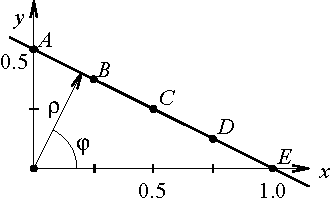
\includegraphics[scale=0.9]{08_segmentace/images/img_8_19.pdf}
    \end{center}
    \caption{Houghova transformace. Body ležící na přímce.}
    \label{img:8_19}
\end{figure}

Pro přímku procházející bodem \textit{Q} reprezentovaným vektorem (\textit{x}$_Q$, \textit{y}$_Q$) pak platí $\rho = x_Q \cos \varphi + y_Q \sin \varphi$. Uvažujme nyní prostor $\varphi$,$\rho$. V tomto prostoru odpovídá každé přímce procházející bodem \textit{Q} jediný bod. Svazku přímek procházejících bodem \textit{Q} pak v tomto prostoru odpovídá sinusoida $\rho$ = \textit{x}$_Q$ cos $\varphi$ + \textit{y}$_Q$ sin $\varphi$. Mějme nyní v obraze např. body \textit{A},\textit{B},\textit{C},\textit{D},\textit{E}, které leží na přímce (obr. \ref{img:8_19}). Svazkům možných přímek v těchto bodech odpovídají v prostoru $\varphi$,$\rho$ sinusoidy \textit{A},\textit{B},\textit{C},\textit{D},\textit{E} (obr. \ref{img:8_20}). Obrazem přímky, na které leží body \textit{A},\textit{B},\textit{C},\textit{D},\textit{E} (tedy přímky, která je společná všem svazkům), je v prostoru $\varphi$,$\rho$ bod, v němž se sinusoidy \textit{A},\textit{B},\textit{C},\textit{D},\textit{E} protínají.

\begin{figure}[th]
    \begin{center}
        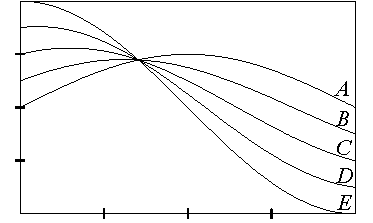
\includegraphics[scale=0.9]{08_segmentace/images/img_8_20.pdf}
    \end{center}
    \caption{Bodům ležícím na přímce odpovídá v prostoru $\varphi$, $\rho$ průsečík sinusoid.}
    \label{img:8_20}
\end{figure}

Dosud provedené úvahy vedou k následujícímu postupu výpočtu. Rozdělme prostor $\varphi$,$\rho$ na oblasti. Nechť např. dvojice (\textit{i},\textit{j}) označuje v prostoru $\varphi$,$\rho$ obdélníkovou oblast, pro niž platí $\varphi_{i-1} \leq \varphi < \varphi_{i}$, $\rho_{j-1} \leq \rho < \rho_j$. Zaveďme nad takto diskretizovaným prostorem $\varphi$,$\rho$ dvourozměrný histogram \textit{h}(\textit{i},\textit{j}). Počáteční hodnota \textit{h}(\textit{i},\textit{j}) je pro všechna (\textit{i},\textit{j}) nula. Nyní probírejme všechny pixely obrazu. Pro každý pixel \textit{Q} = (\textit{x}$_Q$,\textit{y}$_Q$), kde v obraze nalezneme hranu (předpokládáme, že neznáme její směr), sestrojíme v prostoru $\varphi$,$\rho$ sinusoidu (obr. \ref{img:8_21}). Při tom v histogramu inkrementujeme hodnoty \textit{h}(\textit{i},\textit{j}) pro ty oblasti (\textit{i},\textit{j}), kterými sinusoida prochází. Po skončení tohoto procesu \textit{h}(\textit{i},\textit{j}) = \textit{n}  popisuje skutečnost, že na přímce charakterizované hodnotami $\varphi\in\langle\varphi_{i-1}, \varphi_i)$, $\rho\in\langle\rho_{j-1}, \rho_j)$ leží v obraze \textit{n} bodů, které byly považovány za hrany. Pomocí Houghovy transformace tak můžeme zjistit, že v obraze leží v jedné přímce vysoký počet bodů hran. V případě potřeby je toto zjištění možné dále doplnit analýzou, jak jsou detekované body rozloženy podél nalezené přímky.

\begin{figure}[th]
    \begin{center}
        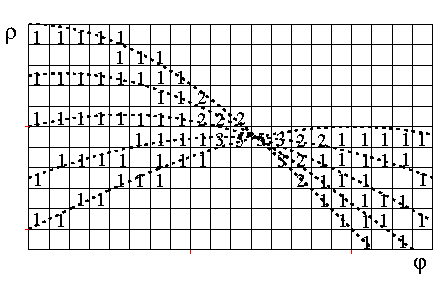
\includegraphics[scale=0.9]{08_segmentace/images/img_8_21.pdf}
    \end{center}
    \caption{Bodům ležícím na přímce odpovídá vysoká hodnota v histogramu.}
    \label{img:8_21}
\end{figure}

Jestliže v~jednotlivých bodech obrazu dokážeme hranu nejen detekovat, ale také dostatečně spolehlivě určit její směr, pak lze popsanou metodu zjednodušit. Nechť (\textit{x},\textit{y}) je bod hrany a $\psi$ směr hrany v tomto bodě. Potom podle vztahu $\rho = x \cos(\psi-\pi/2) + y \sin(\psi-\pi/2)$ můžeme ihned vypočítat odpovídající hodnotu $\rho$. V tomto případě tedy místo generování sinusoidy generujeme pouze jednotlivé body a histogram inkrementujeme pouze v jediné oblasti. Na závěr poznamenejme, že Houghovu transformaci lze zobecnit také na křivky. Protože počet hledaných parametrů křivky udává potřebný rozměr histogramu, jedná nejčastěji o křivky se dvěma, nejvýše třemi parametry.

\section*{Detekce oblastí}

V podkapitole \ref{sec:detekce_hran} jsme popsali metody segmentace obrazu, které byly založeny na detekci hranice oblasti. Jiná skupina metod se zaměřuje přímo na vyhledávání celých oblastí v obraze. Oblasti jsou vyhledávány na základě jistým způsobem zvoleného kriteria homogenity oblasti. Takovým kriteriem mohou být např. konstantní nebo dosti blízké hodnoty jasu, barvy, pokrytí stejnou texturou atd. Protože ze znalosti hranice dokážeme určit také vnitřek oblasti a naopak, zdá se, že by metody založené na detekci hranic i metody založené na detekci celých oblastí měly být vzájemně rovnocenné. Už na obr. \ref{img:8_1} jsme však naznačili, že tomu tak v~praxi nemusí vždy být. Metody založené na detekci oblastí jsou často upřednostňovány u dosti zašumělých obrazů, kde by detekce hranic byla nespolehlivá. Metody detekce oblastí lze rozdělit do tří základních skupin: 1) detekce prahováním, 2) detekce narůstáním oblastí, 3) detekce dělením oblastí. V následujících odstavcích tyto metody popíšeme podrobněji.

\subsection*{Prahování}

Prahování je nejjednodušší metodou detekce celých oblastí v obraze. V nekomplikovaných případech se při tom však současně jedná o metodu rychlou a spolehlivou. Výsledkem prahování je binární obraz, v němž je bodům (pixelům) nalezených oblastí obvykle přiřazena hodnota 1, zatímco zbývajícím bodům (bodům pozadí) je přiřazena hodnota 0. Při prahování se vychází z předpokladu, že body hledaných oblastí mají stejný nebo dosti podobný jas. Jedna z možných realizací prahování spočívá v tom, že pixel je označen jako bod oblasti, jestliže jeho jas padne do intervalu $\langle a, b\rangle$. Velmi často je v rozhodovacím kriteriu použita pouze jediná hodnota \textit{t} - tzv. práh. Body, jejichž jas je vyšší než hodnota prahu, jsou detekovány jako body hledaných oblastí a body, jejichž jas je nižší, jsou detekovány jako body pozadí (případně naopak). Prahování se tedy děje na základě předpisu

\begin{equation} \label{eq:8_68}
    g\left(x,y\right) = \left\{
    \begin{array}{cc}
    1, & f\left(x,y\right) \in \left\langle a,b \right\rangle \\
    0, & \mathrm{jinak}
    \end{array}\right.
    \mathrm{nebo}
    g\left(x,y\right) = \left\{
    \begin{array}{cc}
    1, & f\left(x,y\right) \ge t \\
    0, & \mathrm{jinak}
    \end{array}\right. .
\end{equation}

Úspěšnost prahování závisí na znalosti správné hodnoty prahu. Jestliže tuto hodnotu neznáme, je možné pokusit se ji stanovit na základě informací získaných z obrazu, který má být segmentován. Pro obrazy s bimodálním histogramem (histogramem se dvěma vrcholy) jasu se např. často doporučuje volit jako hodnotu \textit{t} prahu hodnotu, v níž histogram dosahuje mezi oběma vrcholy minima (obr. \ref{img:8_22}). Lze snadno domyslet, že tato heuristická metoda má racionální základ. Předpokládá totiž, že v obraze existují dva druhy pixelů: pixely náležící hledaným oblastem a pixely náležící pozadí. Oba druhy pixelů jsou při tom relativně četné a mají dosti odlišný jas, což v histogramu dává vzniknout zmíněným dvěma vrcholům. Nejsou-li na druhé straně uvedené předpoklady splněny, nemusí být výsledky metody uspokojivé. Ne vždy je také histogram bimodální.

\begin{figure}[th]
    \begin{center}
        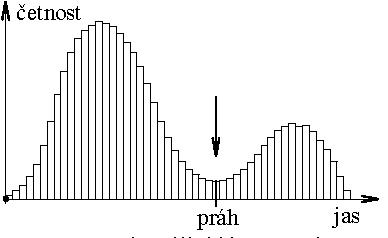
\includegraphics[scale=0.9]{08_segmentace/images/img_8_22.pdf}
    \end{center}
    \caption{Bimodální histogram jasu.}
    \label{img:8_22}
\end{figure}

V případech, kdy je obraz sice kontrastní, avšak v různých svých částech má nerovnoměrnou úroveň jasu, nelze často najít jedinou hodnotu prahu tak, aby vyhovovala pro všechny části obrazu. V takovém případě lze použít prahování s proměnnou hodnotou prahu, kdy se pro různá místa obrazu používá různých hodnot prahu. Metodu lze realizovat tak, že se obraz rozdělí na několik částí a pro každou se najde individuální hodnotu prahu. Je-li histogram úrovní jasů vyšetřované části obrazu bimodální, lze hodnotu prahu stanovit např. postupem popsaným v předchozím odstavci. Jestliže ve vyšetřované části obrazu velmi převažují buď body oblasti nebo body pozadí, pak hodnotu prahu z histogramu uvažované části obrazu spolehlivě stanovit nelze. V takovém případě lze hodnotu prahu stanovit např. jako průměr hodnot prahů z přilehlých oblastí.

\begin{figure}[th]
    \begin{center}
        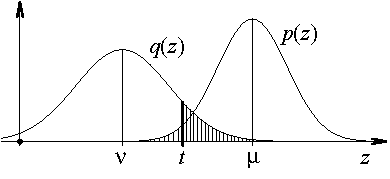
\includegraphics[scale=0.9]{08_segmentace/images/img_8_23.pdf}
    \end{center}
    \caption{Stanovení prahu minimalizací chyby.}
    \label{img:8_23}
\end{figure}

Ukážeme dále důmyslnější metodu stanovení prahu, která je založena na minimalizaci rizika a na využití počtu pravděpodobnosti. Předpokládejme, že jasy pixelů oblastí, které mají být detekovány, mají normální rozložení hustoty pravděpodobnosti \textit{p}(\textit{z}) se střední hodnotou $\mu$ a směrodatnou odchylkou $\sigma$ (obr. \ref{img:8_23}). Podobně předpokládáme, že také jasy pixelů pozadí mají normální rozložení hustoty pravděpodobnosti \textit{q}(\textit{z}) se střední hodnotou $\nu$ a směrodatnou odchylkou $\tau$ (přísně teoreticky vzato nemohou být ovšem rozložení normální, protože prakticky jsou jasové úrovně nenulové pouze v jistém intervalu; může se však jednat o dobré přiblížení). Dále předpokládejme, že podíl pixelů hledaných oblastí na celkovém počtu pixelů obrazu je $\theta$ a že platí $\mu > \nu$. Předpokládejme nyní, že zvolíme práh \textit{t}. Označme \textit{P}(\textit{t}) pravděpodobnost jevu, že bod hledané oblasti bude nesprávně vyhodnocen jako bod pozadí. Dále označme \textit{Q}(\textit{t}) pravděpodobnost jevu, že bod pozadí bude správně vyhodnocen jako bod pozadí. Pak 1 $-$ \textit{Q}(\textit{t}) je pravděpodobnost, že bod pozadí bude nesprávně vyhodnocen jako bod oblasti. Pro pravděpodobnosti \textit{P}(\textit{t}) a \textit{Q}(\textit{t}) máme (obr. \ref{img:8_23})

\begin{equation} \label{eq:8_69}
    P(t) = \int\limits_{-\infty}^{t} p(z)\,dz, \quad Q(t) = \int\limits_{-\infty}^{t} q(z)\,dz .
\end{equation}

Dále musíme uvážit, že poměrné zastoupení bodů objektu v obraze je $\theta$ a poměrné zastoupení bodů pozadí v obraze je ($1-\theta$). Výsledná pravděpodobnost chybné klasifikace je pak

\begin{equation} \label{eq:8_70}
    \varepsilon = \theta P(t) + (1 - \theta)[1 - Q(t)] .
\end{equation}

K nalezení minima výraz \eqref{eq:8_70} derivujeme a derivaci položíme rovnu nule. Dostaneme

\begin{equation} \label{eq:8_71}
    \frac{\partial\varepsilon}{\partial t} = \theta \frac{\partial P(t)}{\partial t} - (1 - \theta) \frac{\partial Q(t)}{\partial t} = \theta p(t) - (1 - Q)q(t) = 0 .
\end{equation}

Odtud máme

\begin{equation} \label{eq:8_72}
    (1 - \theta) q(t) = \theta p(t) .
\end{equation}

Podle předpokladu mají hustoty pravděpodobnosti \textit{p}(\textit{z}) i \textit{q}(\textit{z}) normální rozložení. Je tedy

\begin{equation} \label{eq:8_73}
    p(t) = \frac{1}{\sigma\sqrt{2\pi}} \exp \left[ \frac{-(t - \mu)^2}{2\sigma^2} \right], \quad q(t) = \frac{1}{\tau\sqrt{2\pi}} \exp \left[ \frac{-(t - \nu)^2}{2\tau^2} \right].
\end{equation}

Dosazením vztahů \eqref{eq:8_73} do \eqref{eq:8_72} a logaritmováním máme

\begin{equation} \label{eq:8_74}
    \ln (1 - \tau) - \ln \tau - \frac{(t - \nu)^2}{2\tau^2} = \ln \theta - \ln \sigma - \frac{(t - \mu)^2}{2\sigma^2}.
\end{equation}

Po úpravě dostaneme

\begin{equation} \label{eq:8_75}
    \tau^2 (t - \mu)^2 - \sigma^2 (t - \nu)^2 = 2\sigma^2\tau^2\ln \frac{\tau\theta}{\sigma(1-\theta)}.
\end{equation}

Výraz \eqref{eq:8_75} je kvadratickou rovnicí pro \textit{t}. K řešení je zapotřebí znát hodnoty $\mu$,$\sigma$,$\nu$,$\tau$,$\theta$. Povšimněme si blíže ještě případu, kdy  $\theta$ = 1/2  a  $\sigma$ = $\tau$. V tomto případě se rovnice \eqref{eq:8_75} zjednoduší na tvar

\begin{equation} \label{eq:8_76}
    (t - \mu)^2 = (t - \nu)^2.
\end{equation}

Řešením rovnice \eqref{eq:8_76} je intuitivně očekávaná hodnota \textit{t} = ( $\mu$ + $\nu$ ) / 2.

%\noindent \textbf{8.3.2 Metoda spojování oblastí}

%\noindent Metody založené na spojování začínají pracovat s malými oblastmi (dokonce např. i s jednotlivými pixely), které postupně spojují do větších oblastí. Proces se iterativně opakuje tak dlouho, dokud v~obraze existují oblasti, které lze spojovat. Obvyklými kriterii, která jsou uplatňována při rozhodování, zda lze dvě sousedící oblasti spojit do jediné větší oblasti, jsou následující: Obě oblasti by měly mít stejný nebo podobný jas, barvu, texturu atd. Mezi oběma oblastmi by neměla být zřetelná hrana (existence slabě zřetelné nebo přerušované hrany mezi oběma oblastmi se někdy ale připouští). Spojení oblastí je tím více žádoucí, čím větší je délka, podél níž se oblasti vzájemně dotýkají (délka se měří relativně vzhledem k~rozměrům oblastí). Spojení může být naopak nežádoucí v~případě, že by spojením vznikla oblast nevhodného nebo neočekávaného tvaru. Metodám založeným na spojování oblastí byla v~minulosti věnována značná pozornost. Testování výše uvedených kriterií bylo realizováno různými heuristickými postupy. Metodu spojování oblastí je možné považovat za metodu účinnou. Je však náročnější na implementaci a zpravidla i na výpočetní výkon počítače.

%\noindent \textbf{}

%\noindent \textbf{8.3.3 Metoda dělení oblastí}

%\noindent Tato metoda zpravidla začíná s jedinou oblastí tvořenou celým obrazem a dále opakovaně provádí její dělení na dílčí oblasti. Proces dělení pokračuje tak dlouho, dokud není ve všech vzniklých oblastech dosaženo splnění kriteria homogenity. Dále uvedeme dva příklady kriteria homogenity.

%\noindent Dělení oblasti modální metodou: Často používaným prostředkem k posouzení homogenity oblasti je histogram některé její vlastnosti (např. histogram úrovně jasů). Vychází se z představy, že jestliže histogram obsahuje dva nebo více vrcholů (je bimodální nebo multimodální), pak je vyšetřovaná oblast nehomogenní a je nutné ji rozdělit. K rozdělení lze opět využít znalosti histogramu. Např. u bimodálního histogramu lze za dělící prahovou hodnotu zvolit hodnotu, která odpovídá „údolí`` mezi oběma vrcholy (obr. 8.22). Provedeme-li prahování oblasti s~touto hodnotou prahu, je oblast rozdělena na dvě nebo více nových oblastí. U multimodálních histogramů lze provést dělení buď na základě většího počtu prahů nebo lze vybrat jediný práh odpovídající nejvýznamnějšímu „údolí`` v histogramu a dělení provádět několikrát. Druhý postup bývá považován za spolehlivější. Proces dělení končí, když histogram každé oblasti obsahuje nejvýše jeden vrchol.

%\noindent Dělení oblasti metodou diskriminantu: Existence nehomogenit v oblasti se ne vždy projeví tím, že je histogram (např. jasových úrovní) bimodální. V takovém případě je nutné hledat jiná kriteria. V (Otsu 78) byla např. prezentována metoda, která používá diskriminačního kriteria. Předpokládejme, že pracujeme s úrovněmi jasu 1,2,..., \textit{L}. Uvažujme oblast, která má \textit{n} pixelů. Označme \textit{ni} počet pixelů oblasti, které mají jas \textit{i}. Dále zaveďme \textit{pi} = \textit{ni}/\textit{n}. Střední hodnota a rozptyl jasů v~uvažované oblasti jsou popsány výrazy

% ,     . \eqref{GrindEQ__8_77_}

%\noindent Vysoká hodnota $\sigma$ naznačuje, že je nutné oblast rozdělit. Dělení oblasti provedeme prahováním s~prahem \textit{t}. Stanovení prahu je cílem následující úvahy. Počet pixelů s jasem menším nebo rovným \textit{t} označme \textit{m}1, počet pixelů s~jasem větším než \textit{t} označme \textit{m}2 (\textit{m}1+\textit{ m}2 = \textit{n}). Zaveďme \textit{w}1 = \textit{m}1/\textit{n}, \textit{w}2 = \textit{m}2/\textit{n}. Střední hodnota a rozptyl jasu pro oblasti s~jasem nižším (vyšším) než \textit{t} je

% ,     ,     ,     . \eqref{GrindEQ__8_78_}

%\noindent Pro rozptyl \textit{$\sigma$}2\textit{w} uvnitř tříd a rozptyl \textit{$\sigma$}2\textit{b} mezi třídami platí (Otsu 78)

% ,     . \eqref{GrindEQ__8_79_}

%\noindent Neznámou hodnotu prahu určíme tak, aby minimalizovala $\sigma$2\textit{w} nebo maximalizovala $\sigma$2\textit{b}. Protože platí  $\sigma$2\textit{w} + $\sigma$2\textit{b} = $\sigma$2, jsou obě kriteria ekvivalentní. Nevýhodou této jinak pěkné metody je, že se při stanovení hodnoty prahu nelze vyhnout iteračnímu procesu.

%\noindent 

%\noindent \textbf{8.4 Detekce rohů}

%\noindent 

%\noindent Někdy se další zpracování obrazu může opírat o nalezení rohů (vrcholů) oblastí, což může být výhodné zejména z~následujících důvodů: 1) Rohy bývají bohatě zastoupeny v~obrazech scén vytvořených člověkem i v~obrazech scén „přírodních``. 2) Polohu rohů lze v~obrazech zpravidla jednoznačně určit. 3) Rohy v~obrazech často korespondují s~rohy (vrcholy) skutečných trojdimenzionálních objektů, čehož lze využít např. při rekonstrukci scény. Uvažujme obraz ve stupních šedi a vyšetřujme průběh křivosti plochy popsané obrazovou funkcí. Je zřejmé, že v~místě rohu není křivost v~žádném směru nulová (to je rozdíl ve srovnání s~hranou). Detektory rohů jsou často založeny na uvedeném pozorování. Dále uvedeme dva příklady detektorů. 

%\noindent 

%\noindent \textbf{8.4.1  Kitchen-Rosenfeldův detektor rohů}

%\noindent Tento detektor byl publikován v (Kitchen 82). Nechť \textit{I}(\textit{x},\textit{y}) označuje jas obrazu v bodě \textit{x},\textit{y} a nechť \textit{Ix}, \textit{Iy}, \textit{Ixx}, \textit{Iyy}, \textit{Ixy} jsou derivace funkce \textit{I}. Autoři navrhují v~každém bodě obrazu počítat hodnotu 
%\begin{equation} \label{GrindEQ__8_80_} 
%k=\frac{I_{xx} I_{y}^{2} +I_{yy} I_{x}^{2} -2I_{xy} I_{x} I_{y} }{I_{x}^{2} +I_{y}^{2} }  
%\end{equation} 
%a ukazují, že uvedená hodnota je úměrná velikosti křivosti a velikosti gradientu obrazové funkce v~uvažovaném bodě. Bod (\textit{x},\textit{y}) lze považovat za roh, jestliže je v~něm hodnota \textit{k}~dostatečně vysoká.

%\noindent 

%\noindent \textbf{8.4.2 Harrisův detektor rohů}

%\noindent K novějším detektorům rohů patří detektor navržený Harrisem a Stephensem (Harris 88). V~případě tohoto detektoru konstruujeme v každém bodě obrazu matici
%\begin{equation} \label{GrindEQ__8_81_} 
%M\left(x,y\right)=\left[\begin{array}{cc} {\left\langle \left(I_{x} \right)^{2} \right\rangle } & {\left\langle I_{x} I_{y} \right\rangle } \\ {\left\langle I_{x} I_{y} \right\rangle } & {\left\langle \left(I_{y} \right)^{2} \right\rangle } \end{array}\right].  
%\end{equation} 
%Lomené závorky označují konvoluci s Gaussovou funkcí:
%\begin{equation} \label{GrindEQ__8_82_} 
%\left\langle {\rm y}\left(x,y\right)\right\rangle ={\rm y}\left(x,y\right)*\left[G\left(x\right)G\left(y\right)\right],  
%\end{equation} 
%kde znak * označuje konvoluci a \textit{G}(\textit{u}) je Gaussova funkce
%\begin{equation} \label{GrindEQ__8_83_} 
%G\left(u\right)=\frac{1}{\sqrt{2\pi } \sigma } \exp \left(-\frac{u^{2} }{2\sigma ^{2} } \right). 
%\end{equation} 
%Volba hodnoty $\sigma$ ovlivňuje citlivost detektoru. Derivace ve vztahu \eqref{GrindEQ__8_81_} jsou v praxi aproximovány diferencemi. K rozhodnutí, zda daný bod (\textit{x},\textit{y}) lze považovat za roh, lze využít funkce (Harris 88)
%\begin{equation} \label{GrindEQ__8_84_} 
%{\rm cor}\left(x,y\right)={\rm det}\left(M\left(x,y\right)\right)-0.04\cdot {\rm trace}^{2} \left(M\left(x,y\right)\right).  
%\end{equation} 
%Bod (\textit{x},\textit{y}) považujeme za roh, jestliže jsou splněny následující dvě podmínky: 1) cor(\textit{x},\textit{y}) je větší než nějaká předem stanovená hodnota; 2) hodnota cor(\textit{x},\textit{y}) je největší v okně o předem definovaných rozměrech (okno je svým prostředním pixelem umístěno do bodu (\textit{x},\textit{y})).

%\noindent 

\section*{Zpracování binárních obrazů} \label{sec:zpracovani_binarnich_obrazu}

Binárním obrazem nazýváme takový obraz, v němž obrazová funkce v každém bodě (v každém pixelu) nabývá jedné ze dvou možných hodnot. Binární obrazy jsou zpravidla výsledkem metod provádějících segmentaci obrazu (v pixelech náležících objektům např. obrazová funkce nabývá hodnoty 1, v pixelech pozadí nabývá hodnoty 0). Před tím, než jsou binární obrazy analyzovány, lze je zpracovat některým ze speciálních postupů, které dále ve stručném přehledu popíšeme. 

\subsection*{Matematická morfologie}

Tvůrcem matematické morfologie je Serra (Serra 82). Z poměrně nedávných publikací zabývajících se touto problematikou uveďme alespoň práci (Dougherty 92). Teorie matematické morfologie je dosti obsáhlá, a proto můžeme v tomto textu uvést pouze základní informace. Označme \textbf{B} vstupní binární obraz. Dále budeme pracovat s pomocným binárním obrazem \textbf{S}. Význam tohoto pomocného obrazu bude obdobný jako význam masky u konvoluce - budeme jej postupně přikládat na různá místa obrazu \textbf{B}. Označení \textbf{S}\textit{xy} budeme používat pro obraz, který vznikne translací pomocného obrazu \textbf{S} tak, aby počátek obrazu \textbf{S} padl do bodu o souřadnicích (\textit{x},\textit{y}) (obr. \ref{img:8_24}).  Základními operacemi matematické morfologie jsou \textit{eroze} a \textit{dilatace}. Tyto operace jsou definovány následujícími vztahy (obr. \ref{img:8_25})

\begin{equation} \label{eq:8_85}
    \mathbf{E} = \mathbf{B} \otimes \mathbf{S} = \left\{ x, y | \mathbf{S}_{x, y} \subseteq \mathbf{B} \right\},
\end{equation}

\begin{equation} \label{eq:8_86}
    \mathbf{D} = \mathbf{B} \oplus \mathbf{S} = \left\{ x, y | \mathbf{S}_{x, y} \cap \mathbf{B} \neq \oslash \right\}.
\end{equation}

\begin{figure}[th]
    \begin{center}
        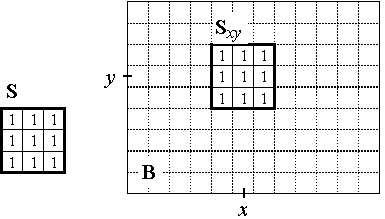
\includegraphics[scale=0.9]{08_segmentace/images/img_8_24.pdf}
    \end{center}
    \caption{K významu masky u morfologických operací.}
    \label{img:8_24}
\end{figure}

Vysvětleme podrobněji význam vztahu \eqref{eq:8_85}. Erozí binárního obrazu \textbf{B} za použití masky \textbf{S} vznikne obraz \textbf{E}, který je opět binární. Předpokládejme, že jednotlivé body binárního obrazu nesou hodnotu 0 nebo 1. V bodě o souřadnicích (\textit{x},\textit{y}) je v obraze \textbf{E} hodnota 1, jestliže je v obraze \textbf{B} hodnota 1 alespoň na těch místech, kde je hodnota 1 v masce  \textbf{S}$_{xy}$. Jinak je v obraze \textbf{E} v bodě o souřadnicích (\textit{x},\textit{y}) hodnota 0. Ve vztahu \eqref{eq:8_85} jsou obrazy formálně reprezentovány jako množiny - jedná se o množiny pixelů nesoucích hodnotu 1. Analogicky by bylo možné interpretovat také vztah \eqref{eq:8_86}. 

Dalšími často používanými operacemi matematické morfologie jsou otevření a uzávěr. Otevření je definováno jako eroze následovaná dilatací (vztah 8.87). Uzavření je naopak dilatace následovaná erozí (vztah 8.88). Máme tedy

\begin{equation} \label{eq:8_87}
    \mathbf{B} \circ \mathbf{S} = \left( \mathbf{B} \otimes \mathbf{S} \right) \oplus \mathbf{S},
\end{equation}

\begin{equation} \label{eq:8_88}
    \mathbf{B} \bullet \mathbf{S} = \left( \mathbf{B} \oplus \mathbf{S} \right) \times \mathbf{S}.
\end{equation}

Z definice je zřejmé, že otevření eliminuje malé a tenké objekty a rozděluje objekty v místech, kde jsou tenké. Uzavření naopak vyplňuje malé a tenké díry v objektech a spojuje objekty, které leží blízko sebe. Poznamenejme, že někdy může být výhodné použít většího počtu otevření nebo uzavření po sobě. Alternativně může také být otevření a uzavření realizováno tak, že je použito většího počtu operací eroze a stejného počtu operací dilatace.

\begin{figure}[th]
    \begin{center}
        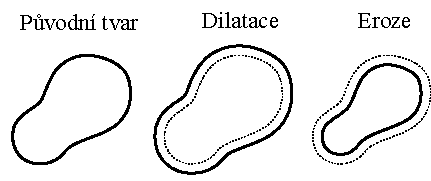
\includegraphics[scale=0.9]{08_segmentace/images/img_8_25.pdf}
    \end{center}
    \caption{Dilatace a eroze.}
    \label{img:8_25}
\end{figure}

\subsection*{Ztenčování}

Cílem ztenčování je reprezentovat objekty v~obraze jako lineární útvary (obr. \ref{img:8_26}). Ztenčování může být realizováno pomocí opakovaně prováděné eroze (tj. opakovaným odstraňováním krajních pixelů z~objektu). Postup provádění každého erozního kroku je při tom modifikován tak, aby nedošlo k~porušení souvislosti objektu. Při praktickém výpočtu jsou dle vztahu \eqref{eq:8_85} nejprve detekovány pixely objektu kandidující na to, že do nich bude zapsána hodnota 0 (tj. budou z objektu odstraněny). Tato hodnota je pak ale skutečně zapsána jen do některých z~kandidujícíh pixelů. Pixely jsou vybrány tak, aby zápisem hodnoty 0 nedošlo k~rozdělení zbývající části objektu na více částí. Proces opakovaného provádění eroze pokračuje tak dlouho, dokud lze nějaké pixely odstraňovat.

\begin{figure}[th]
    \begin{center}
        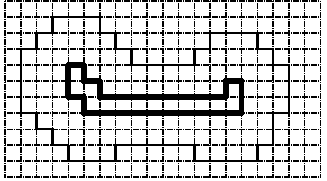
\includegraphics[scale=0.9]{08_segmentace/images/img_8_26.pdf}
    \end{center}
    \caption{Obrázek před a po ztenčení.}
    \label{img:8_26}
\end{figure}

\subsection*{Kostra}

Také v~případě kostry je cílem popsat tvar plošného objektu pomocí lineárních útvarů. Často se uvádí (Fu 86, Castleman 96) následující neformální definice kostry: Představme si oblast, jejíž kostru hledáme, jako trávník. Jestliže trávník po celém jeho okraji zapálíme a bude-li se oheň šířit všemi směry stejnou rychlostí, pak množinu bodů, kde se setkají „různé ohně`` nazveme kostrou. Kostrou oblasti ve tvaru kruhu je jeho střed. Příklad na obr. \ref{img:8_27}a ukazuje kostru obdélníka. Na obr. \ref{img:8_27}b je uveden příklad naznačující obtíže, které vzniknou při doslovné aplikaci dříve uvedené definice kostry. Ačkoli malý výstupek na pravé straně obdélníka může být pouhou nepřesností způsobenou digitalizací, výsledná kostra se dosti liší od kostry ideálního obdélníka. Při praktické implementaci algoritmů pro stanovení kostry je zpravidla zapotřebí  tyto jevy potlačit.

\begin{figure}[th]
    \begin{center}
        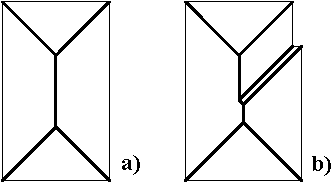
\includegraphics[scale=0.9]{08_segmentace/images/img_8_27.pdf}
    \end{center}
    \caption{a) Kostra obdélníka. b) Vliv chyby způsobené digitalizací.}
    \label{img:8_27}
\end{figure}

%\noindent 

%\subsection*{Indexování}

%\noindent Pro další zpracování binárního obrazu může být někdy výhodné provést tzv. indexování oblastí. Indexováním rozumíme, že každé oblasti (každému rozpoznávanému objektu) je přiřazeno přirozené číslo, které je pak zapsáno do každého pixelu oblasti (obr.8.28). Za jednu oblast při tom považujeme množinu vzájemně sousedících pixelů, v nichž byla v původním binárním obraze zapsána hodnota 1. Při rozhodování, zda pixely sousedí, rozlišujeme tzv. \textit{čtyřsousednost} a \textit{osmisousednost}. Představme si  pixely jako čtverečky podobně, jak je vyobrazeno na obr. 8.28. Při čtyřsousednosti považujeme dva pixely za sousedící, jestliže mají společnou stranu. Každý pixel tak má čtyři sousedy. V případě osmisousednosti považujeme za sousedy pixelu všech osm pixelů, které s daným pixelem sousedí hranou nebo pouze rohem. Indexovaného obrazu lze využít např. při praktické implementaci výpočtu atributů objektů při příznakovém rozpoznávání.
